\documentclass[12pt,a4paper]{article}
\usepackage[utf8]{inputenc}
\usepackage[T2A]{fontenc}
\usepackage[ukrainian]{babel}
\usepackage{fancyvrb}
\usepackage{pdflscape}

\usepackage{amsmath} % у преамбулі
\usepackage{array, multirow}
\usepackage{hyperref} % <-- Обов’язково підключіть цей пакет
\usepackage{caption}
\usepackage{booktabs}

\usepackage{xcolor}

\renewcommand{\thetable}{№\arabic{table}}
\captionsetup[table]{name=Таблиця}  % замість "Табл." буде "Таблиця"

\usepackage{graphicx} % <-- Для роботи з \includegraphics
\usepackage{geometry}
\geometry{
    left=2cm,
    right=2cm,
    top=2cm,
    bottom=2cm
}

\begin{document}

    \begin{titlepage}

        \thispagestyle{empty}
        \begin{center}
        \large
        Національний технічний університет України\\
        «Київський політехнічний інститут імені Ігоря Сікорського»\\[1em]
        Факультет інформатики та обчислювальної техніки\\
        Кафедра загальної фізики
        \end{center}

        \vfill

        \begin{center}
        \textbf{\LARGE Фізика}\\[2em]
        \textbf{\Large Лабораторна робота №ФПЕ-11}\\
        «Вивчення вимушених коливань у коливальному контурі» 
        \end{center}

        \vfill

        \begin{flushright}
        Виконав: студент 1 курсу ФІОТ, гр. ІО-41\\
        \textit{Давидчук А. М.}\\
        Залікова книжка № 4106\\[1em]
        Перевірив: \textit{Колган В.\,В.}
        \end{flushright}

        \vfill

        \begin{center}
        Київ -- 2025
        \end{center}

    \end{titlepage}

    \setlength{\parindent}{0pt}

    \textbf{\underline{Тема:}} «Вивчення вимушених коливань у коливальному контурі».

    \vspace{1em}

    \textbf{Мета:} вивчення резонансу у послідовному колі $R$, $C$, $L$.

    \vspace{1em}

    \textbf{\underline{Прилади та обладнання (рис. 4.1):}}
    РQ – звуковий генератор ГЗ-102; РО – електронний осцилограф С1-75;
    ФПЭ-11 – касета ФПЕ-11; МО – магазин опорів; МЄ – магазин ємностей.

    \begin{figure}[h!]

        \renewcommand{\thefigure}{4.\arabic{figure}} % робимо "3.1", "3.2" і т.д.

        \centering
        % Підставляєте потрібний шлях та розмір зображення:
        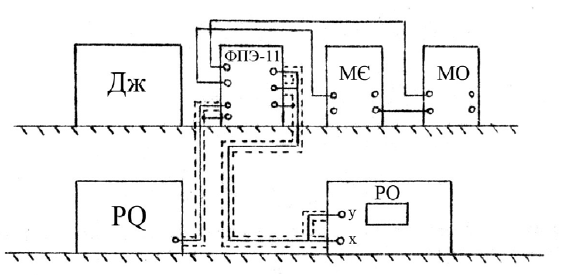
\includegraphics[width=0.6\textwidth]{main_schemma.png}
        % Підпис (зазвичай під малюнком):
        \caption{Загальна схема досліду}
        % Мітка для посилань у тексті (\ref{fig:...})
        \label{fig1:schema}

    \end{figure}

    %%%%%%%%%%%%%%%%%%                      Теоритчні відомості                         %%%%%%%%%%%%%%%%%%%%%%%

    \begin{center}
        \textbf{\Large Теоретичні відомості}
    \end{center}

    \setlength{\parindent}{1.5em}

    Розглянемо процеси, які проходять у послідовному коливальному контурі, приєднаному до джерела, електрорушійна сила якого змінюється з часом за гармонічним законом

    \begin{equation}
        \mathcal{E} = \mathcal{E}_0 \cos \Omega t
        \tag{4.1}
    \end{equation}

    Введемо такі позначення:
    $U$ --- напруга на конденсаторі ємністю $C$,
    $U_L$ --- напруга на котушці індуктивності, $I$ --- сила струму у контурі.
    Якщо вважати миттєві значення струмів та напруг однаковими на усіх ділянках кола
    (квазістаціонарний струм), то струм і напруга в контурі будуть підпорядковані законам,
    встановленим для сталого струму. За другим правилом Кірхгофа сума напруг на елементах контуру дорівнює ЕРС, що діє в цьому ж контурі (рис. 4.2).
    
    \begin{figure}[h!]

        \renewcommand{\thefigure}{4.\arabic{figure}} % робимо "3.1", "3.2" і т.д.

        \centering
        % Підставляєте потрібний шлях та розмір зображення:
        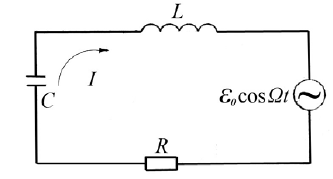
\includegraphics[width=0.5\textwidth]{4.2.png}
        % Підпис (зазвичай під малюнком):
        \caption{Схема коливального контуру}
        % Мітка для посилань у тексті (\ref{fig:...})
        \label{fig2:schema}

    \end{figure}

    Таким чином, можемо записати:

    \begin{equation}
        U_L + IR + U = \mathcal{E}_0 \cos \Omega t
        \tag{4.2}
    \end{equation}

    Напруга на котушці чисельно дорівнює ЕРС самоіндукції

    \begin{equation}
        U_L = -\mathcal{E}_i = L \frac{dI}{dt}
        \tag{4.3}
    \end{equation}

    Струм у колі визначає зміну заряду конденсатора, тому

    \vspace{0.5em}

    \begin{equation}
        I = \frac{dq}{dt} = \frac{d(CU)}{dt} = C \frac{dU}{dt}
        \tag{4.4}
    \end{equation}

    \vspace{0.5em}

    Підставивши (4.3) в (4.4) в (4.2), отримаємо

    \vspace{0.5em}

    \begin{equation}
        LC \frac{d^2U}{dt^2} + RC \frac{dU}{dt} + U = \mathcal{E}_0 \cos \Omega t
        \tag{4.5}
    \end{equation}

    \vspace{0.5em}

    Розділимо всі частини рівняння $LC$

    \vspace{0.5em}

    \begin{center}
        $\displaystyle \frac{d^2U}{dt^2} + \frac{R}{L} \frac{dU}{dt} + \frac{1}{LC}U = \mathcal{E}_0 \cos \Omega t$
    \end{center}

    \vspace{0.5em}

    Введемо такі позначення

    \vspace{0.5em}

    \begin{center}
        $\displaystyle \omega_0^2 = \frac{1}{LC}; \quad \beta = \frac{R}{2L}$.
    \end{center}

    Представимо рівняння (4.5) у канонічній формі

    \vspace{0.5em}

    \begin{equation}
        \frac{d^2U}{dt^2} + 2\beta \frac{dU}{dt} + \omega_0^2 U = \mathcal{E}_0 \omega_0^2 \cos \Omega t
        \tag{4.6}
    \end{equation}

    \vspace{0.5em}

    Розв’язуючи рівняння (4.6), отримуємо закон зміни напруги на конденсаторі з часом. Розв’язок неоднорідного диференціального рівняння другого порядку (4.6) дорівнює сумі повного розв’язку відповідного однорідного рівняння (4.7) та частинного розв’язку неоднорідного
    рівняння (4.6).

    \vspace{0.5em}

    \begin{equation}
        \frac{d^2U}{dt^2} + 2 \beta \frac{dU}{dt} + \omega_0^2 U = 0.
        \tag{4.7}
    \end{equation}

    \vspace{0.5em}

    За умови, що $\omega_0^2 > \beta^2$ розв’язком рівняння (4.7) є функція

    \vspace{0.5em}

    \begin{equation}
        U_1 = U_{10} e^{-\beta t} \cos \omega t.
        \tag{4.8}
    \end{equation}

    \vspace{0.5em}

    Це – рівняння загасаючих коливань
    (див. лабораторну роботу 3 (ФПЕ-10)).
    Загасання визначається множником $e^{-\beta t}$.
    За час $\tau = 1/\beta$, який називають часом релаксації,
    амплітуда коливань зменшується в $e$ разів.
    Загасання коливань у контурі зумовлено нагріванням провідників,
    тобто перетворенням енергії електричного та магнітного полів
    на теплову (внутрішню) енергію.
    Складова визначає перехідний процес при встановленні коливань,
    Якщо ж $t >> \tau$, то ця складова в загальному розв’язку зникає.
    Під дією джерела змінної ЕРС в колі встановлюються коливання
    з частотою цього джерела, але із зсувом фаз

    \vspace{0.5em}

    \begin{equation}
        U = U_0 \cos (\Omega t + \varphi)
        \tag{4.9}
    \end{equation}

    \vspace{0.5em}

    Підставляючи (4.9) в (4.6) матимемо

    \begin{equation}
        U_0 = \frac{\mathcal{E}_0 \omega_0^2}{\sqrt{\left(\omega_0^2 - \Omega^2 \right)^2 + 4\beta^2\Omega^2}}
        \tag{4.10}
    \end{equation}

    \begin{equation}
        \tg \varphi = -\frac{2\beta \Omega}{\omega_0^2 - \Omega^2}
        \tag{4.11}
    \end{equation}

    \vspace{0.5em}

    Отже, амплітуда та фаза напруги на конденсаторі,
    а також амплітуда сили струму в контурі залежать
    від співвідношення частоти джерела ЕРС $\Omega$ та частоти
    $\displaystyle \omega_0^2 = \frac{1}{LC}$

    Струм в контурі

    \vspace{0.5em}

    \begin{center}
        $\displaystyle I = C\frac{dU}{dt} = -\Omega C U_0 \sin(\Omega t + \varphi) = I_0 \cos(\Omega t + \varphi_1)$.
    \end{center}

    де $\varphi_1 = \varphi + \pi/2$.

    Амплітуда сили струму

    \vspace{0.5em}

    \begin{equation}
        I_0 = \frac{\mathcal{E}_0 C \omega_0^2 \Omega}{\sqrt{\left(\omega_0^2 - \Omega^2 \right)^2 + 4\beta^2\Omega^2}}
        \tag{4.12}
    \end{equation}

    \vspace{0.5em}

    Графік залежності $I_0$ від $\Omega / \omega_0$ зображено на рис. 4.3.

    \begin{figure}[h!]

        \renewcommand{\thefigure}{4.\arabic{figure}} % робимо "3.1", "3.2" і т.д.

        \centering
        % Підставляєте потрібний шлях та розмір зображення:
        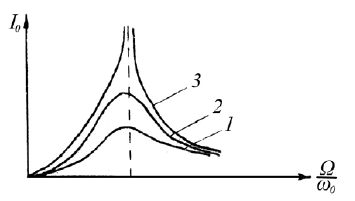
\includegraphics[width=0.5\textwidth]{4.3.png}
        % Підпис (зазвичай під малюнком):
        \caption{Резонансні криві}
        % Мітка для посилань у тексті (\ref{fig:...})
        \label{fig3:schema}

    \end{figure}

    З графіка видно, що амплітуда сили струму різко зростає,
    якщо кутова частота $\Omega$ джерела ЕРС наближається до частоти
    $\omega_0$. Це явище називається резонансом в електричному колі,
    а криві --- резонансними кривими.
    Значення максимуму сили струму залежить від
    $\beta$: при $\beta = 0$, $I_0 \rightarrow \infty$ (крива 3);
    при збільшенні $\beta$ максимальне значення $I_0$ зменшується (криві 1, 2).

    Кут $\varphi_1$ визначає різницю фаз коливань сили струму у контурі та зовнішньої ЕРС:

    \vspace{0.5em}

    \begin{equation}
        \tg \varphi_1 = \tg \left( \varphi + \frac{\pi}{2} \right) = - \frac{1}{\tg \varphi} = \frac{\omega_0^2 - \Omega^2}{2\beta \Omega}
        \tag{4.13}
    \end{equation}

    \vspace{0.5em}

    Графік залежності $\varphi_1$ від частоти $\Omega$ зображено на
    рис. 4.4.

    \newpage

    \begin{figure}[h!]

        \renewcommand{\thefigure}{4.\arabic{figure}} % робимо "3.1", "3.2" і т.д.

        \centering
        % Підставляєте потрібний шлях та розмір зображення:
        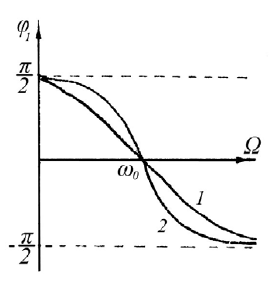
\includegraphics[width=0.3\textwidth]{4.4.png}
        % Підпис (зазвичай під малюнком):
        \caption{Залежність різниці фаз коливань сили струму в контурі та зовнішньої ЕРС від частоти зовнішньої ЕРС.}
        % Мітка для посилань у тексті (\ref{fig:...})
        \label{fig4:schema}

    \end{figure}
    
    Криві 1 та 2 відповідають різним значенням $\beta$.
    При $\Omega = \omega_0$, $\tg \varphi_1 = 0$ та $\varphi_1 = 0$.

    Величина $\Omega = \omega / (2 \beta)$ (тут $\omega = \sqrt{\omega_0^2 - \beta^2}$ --- циклічна частота загасаючих коливань)
    називається добротністю коливального контуру.
    Добротність контуру визначається гостротою резонансних кривих.
    Знайдемо ширину резонансної кривої $\Delta \Omega$ на
    рівні $I_0 = I_{0_{max}} / \sqrt{2}$ (рис. 4.5).

    \begin{figure}[h!]

        \renewcommand{\thefigure}{4.\arabic{figure}} % робимо "3.1", "3.2" і т.д.

        \centering
        % Підставляєте потрібний шлях та розмір зображення:
        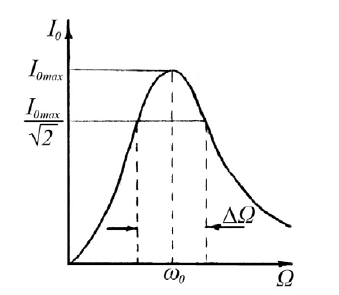
\includegraphics[width=0.4\textwidth]{4.5.png}
        % Підпис (зазвичай під малюнком):
        \caption{Визначення добротності контуру за шириною резо-нансної кривої.}
        % Мітка для посилань у тексті (\ref{fig:...})
        \label{fig5:schema}

    \end{figure}

    З формули (4.12) випливає,
    що максимальне значення сили струму $\displaystyle I_{0_{max}} = \frac{\mathcal{E}_0 C \omega_0^2}{2\beta}$,
    а

    \vspace{0.5em}

    \begin{equation}
        I_0 = \frac{2\beta \Omega I_{0_{max}}}{\sqrt{\left(\omega_0^2 - \Omega^2 \right)^2 + 4\beta \Omega^2}}
        \tag{4.14}
    \end{equation}

    \vspace{0.5em}

    За умови $I_0 = I_{0_{max}} / \sqrt{2}$ формула (4.14) матиме вигляд:

    \vspace{0.5em}

    \begin{equation}
        \frac{1}{\sqrt{2}} = \frac{2\beta \Omega}{\sqrt{\left(\omega_0^2 - \Omega^2 \right)^2 + 4\beta \Omega^2}}
        \tag{4.15}
    \end{equation}

    \vspace{0.5em}

    Вираз (4.15) можна перетворити таким чином

    \vspace{0.5em}

    \begin{center}
        $\displaystyle 2\beta \Omega = \omega_0^2 - \Omega^2$
    \end{center}

    \vspace{0.5em}

    або $2\beta \Omega = (\omega_0 - \Omega)(\omega_0 + \Omega)$.
    Величина $\omega_0 - \Omega = \Delta \Omega / 2$, а
    поблизу резонансу $\omega_0 \approx \Omega$.
    Після підстановки отримаємо, що $\Delta \Omega = 2\beta$.

    \vspace{0.5em}

    \begin{equation}
        \frac{\Delta \Omega}{\omega_0} = \frac{2 \beta}{\omega_0} \approx \frac{1}{Q}
        \tag{4.16}
    \end{equation}

    \vspace{0.5em}

    За умов малого загасання виконуються
    співвідношення $\beta << \omega_0$ і $\omega \approx \omega_0$, а відносна ширина
    резонансної кривої чисельно дорівнює величині,
    яка обернено пропорційна добротності контуру.
    Якщо відомі параметри коливального контуру,
    то добротність може бути розрахована за формулою

    \vspace{0.5em}

    \begin{equation}
        Q = \frac{\omega_0}{2\beta} = \frac{1}{R} \sqrt{\frac{L}{C}}.
        \tag{4.16а}
    \end{equation}

    \vspace{0.5em}

    Принципова електрична схема експериментальної установки показана на рис. 4.6.

    \begin{figure}[h!]

        \renewcommand{\thefigure}{4.\arabic{figure}} % робимо "3.1", "3.2" і т.д.

        \centering
        % Підставляєте потрібний шлях та розмір зображення:
        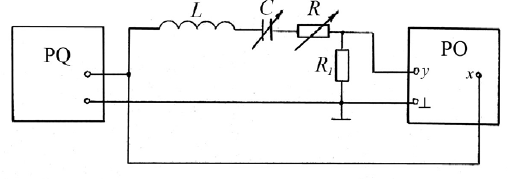
\includegraphics[width=0.5\textwidth]{4.6.png}
        % Підпис (зазвичай під малюнком):
        \caption{Принципова електрична схема експериментальної установки.}
        % Мітка для посилань у тексті (\ref{fig:...})
        \label{fig6:schema}

    \end{figure}

    Коливальний контур складається з котушки $L$,
    магазину ємностей $C$, змінного резистора $R$ та резистора $R_1$.
    Напруга на резисторі $R_1$, яка пропорційна силі струму у контурі,
    подається на вхід "Y" електронного осцилографа, а сигнал звукового генератора --- на вхід “X”. Для зняття резонансних кривих, змінюючи
    частоту звукового генератора PQ, вимірюють залежність сили струму в контурі від частоти генератора $I_0 = f(\Omega)$ при різних значеннях опору резистора $R$.

    Для вимірювання зсуву фаз $\varphi$ використовують фігури Ліссажу,
    які отримують на екрані осцилографа
    Нехай є дві синусоїдні напруги однакової частоти $\Omega$.
    Якщо їх подати на вертикальні і горизонтальні відхиляючі
    пластини осцилографа, то
    відбудуться відповідні зміщення електронного променя на екрані:

    \vspace{0.5em}

    \begin{center}
        \begin{tabular}{ll}
            по горизонталі & \( x = x_0 \cos \Omega t, \) \\
            по вертикалі   & \( y = y_0 \cos(\Omega t + \varphi), \)
        \end{tabular}
    \end{center}

    де $\varphi$ --- зсув фаз між напругами; $x_0$ та $y_0$ --- амплітуди зміщення променя,
    які пропорційні амплітудам напруги та коефіцієнтам
    підсилення відповідних каналів осцилографа.
    Виключивши час з двох останніх рівнянь, отримаємо

    \vspace{0.5em}

    \begin{equation}
        \left( \frac{x}{x_0} \right)^2 + \left( \frac{y}{y_0} \right)^2 - \frac{2xy}{x_0 y_0} \cos \varphi = \sin^2 \varphi.
        \tag{4.17}
    \end{equation}

    \vspace{0.5em}

    Вираз (4.17) є рівнянням еліпса, який описується електронним
    променем на екрані осцилографа.
    Якщо коефіцієнти підсилення підібрати так,
    щоб задовольнялася рівність $x_0 = y_0$, то рівняння (4.17)
    набуде вигляду

    \vspace{0.5em}

    \begin{equation}
        x^2 + y^2 -2xy \cos \varphi = x_0^2 \sin^2 \varphi.
        \tag{4.18}
    \end{equation}

    \vspace{0.5em}

    Формула (4.18) --- рівняння еліпса, осі якого утворюють кути
    $4\pi$ з осями координат.
    При $\varphi = 0$ еліпс вироджується в пряму $y = x$,
    а при $\varphi = \pi / 2$ --- в коло радіуса $x_0 = y_0$ (рис. 4.7).

    \begin{figure}[h!]

        \renewcommand{\thefigure}{4.\arabic{figure}} % робимо "3.1", "3.2" і т.д.

        \centering
        % Підставляєте потрібний шлях та розмір зображення:
        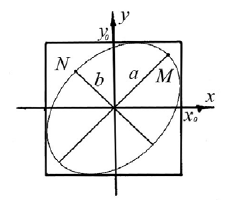
\includegraphics[width=0.5\textwidth]{4.7.png}
        % Підпис (зазвичай під малюнком):
        \caption{Фігура Ліссажу.}
        % Мітка для посилань у тексті (\ref{fig:...})
        \label{fig7:schema}

    \end{figure}

    Для точки $M$ еліпса $y = x$, відповідно $a^2 + x^2 + y^2 = 2x^2$,
    отже рівняння (4.18) для цієї точки матиме вигляд:

    \begin{center}
        $2x^2 - 2x^2 \cos \varphi = x_0^2 \sin^2 \varphi$, \\ \vspace{0.3em}
        $2x^2 (1 - \cos \varphi) = x_0^2 \sin^2 \varphi$, \\ \vspace{0.3em}
        $2a^2 \sin^2 \frac{\varphi}{2} = 4x_0^2 \sin^2 \frac{\varphi}{2} \cos^2 \frac{\varphi}{2}$.
    \end{center}

    Звідки

    \vspace{0.5em}

    \begin{equation}
        a^2 = 2x_0^2 \cos^2 \frac{\varphi}{2}.
        \tag{4.19}
    \end{equation}

    \vspace{0.5em}

    Аналогічно для точки $N$ еліпса, де $y = -x$ (рис. 4.7), можна одержати

    \vspace{0.5em}

    \begin{equation}
        b^2 = 2x_0^2 \sin^2 \frac{\varphi}{2}.
        \tag{4.20}
    \end{equation}

    \vspace{0.5em}

    З виразів (4.19) та (4.20) маємо

    \vspace{0.5em}

    \begin{equation}
        \tg \frac{\varphi}{2} = \frac{b}{a}.
        \tag{4.21}
    \end{equation}

    \vspace{0.5em}

    Таким чином, для визначення зсуву фаз між напругами однакової
    частоти достатньо виміряти півосі еліпса $a$ та $b$ на
    екрані осцилографа.
    Зсув фаз $\varphi$ може бути розрахований за формулою
    (4.18).

    Для отримання фігур Ліссажу на вхід "Y" осцилографа подається
    напруга з резистора $R_1$, яка пропорційна силі струму, а на вхід
    "X" --- напруга зі звукового генератора.
    В результаті вимірювань та розрахунків за формулою
    (4.21) отримуємо кут $\varphi_1$ --- зсув фаз між струмом у
    контурі та зовнішньою ЕРС.

    \newpage

    %%%%%%%%%%%%%%%%%%                      Практична частина                         %%%%%%%%%%%%%%%%%%%%%%%

    \setlength{\parindent}{0pt}

    \begin{center}
        \textbf{\Large Практична частина}
    \end{center}

    \textbf{Порядок виконання завдання №1 (Зняття резонансних кривих):}

    \begin{enumerate}
        \item Перевірив правильність зібраної електричної схеми (рис. 4.8).
    
        \item Встановив початкові значення: ємність $C = 3\cdot10^{-3}$ мкФ, опір $R = 1$ Ом.
    
        \item Увімкнув прилади, подав сигнал частотою 10 кГц на осцилограф і налаштував чітке зображення синусоїди.
    
        \item Плавно змінюючи частоту генератора, визначив резонансну частоту $f_{\text{рез}}$.
    
        \item Виміряв кількість поділок $A$ на піку, та зафіксував значення коефіцієт розшиерння $K_y$ синусоїди для частот від 2 до 16 кГц (крок 2 кГц, поблизу резонансу – 0,2 кГц), розрахував значення амплітуди струму:

        \vspace{-0.5em}

        \begin{center}
            $\displaystyle I_0 = \frac{K_y \cdot A}{R_1}, \quad R_1 = 100$ Ом
        \end{center}

        \vspace{-0.5em}

        результати заніс у таблицю.
    
        \item Повторив вимірювання для значень опору $R = 500$ Ом і $R = 3000$ Ом, результати заніс у таблицю.
    
        \item Побудував графіки залежності амплітуди струму $I_0$ від частоти $f$ для трьох значень опору.
    
        \item За графіком визначив ширину резонансної кривої $\Delta f$ на рівні $I_{0 max}/\sqrt{2}$ для опорів $R = 1$ Ом та $R = 500$ Ом, обчислив добротність:
        
        \begin{equation}
            Q = \frac{f_{\text{рез}}}{\Delta f}
            \tag{4.п1}
        \end{equation}

    \end{enumerate}

    \textbf{Порядок виконання завдання №2 (Визначення залежності резонансної частоти від ємності):}

    \begin{enumerate}

        \item Встановив ємність $C = 1\cdot10^{-3}$ мкФ, опір $R = 1$ Ом, перемикач осцилографа в режим «X».
    
        \item Змінюючи частоту, домігся перетворення фігури Ліссажу (еліпса) на пряму під кутом $45^{\circ}$, визначив резонансну частоту.
    
        \item Повторив вимірювання для значень ємності від $1\cdot10^{-3}$ до $1\cdot10^{-2}$ мкФ, результати заніс у таблицю.
    
        \item Розрахував величини:

        \vspace{-0.5em}

        \begin{center}
            $\displaystyle Z = (2\pi f_{\text{рез}})^2$,
        \end{center}

        \vspace{-0.5em}

        побудував графік залежності $Z(C)$ з урахуванням похибок вимірювання $C$ в 5\%.
    
        \item За коефіцієнтами нахилу, визначив значення котушки $L_1$, $L_2$, та з них, $L_{\text{ср}}$:

        \begin{center}
            $\displaystyle L = \frac{\Delta Z}{\Delta C}, \quad L_{cp} = \frac{L_1 + L_2}{2}$,
        \end{center}

    \end{enumerate}

    Для всіх виміряних значень розрахував похибку вимірювань. Для громіздких обчислень я використовував Python (див. Лістинги 4.1, 4.2 та 4.3).

    \textbf{Всі вимірювання проводив у симуляторі лабораторної роботи ФПЕ-11 (FPE11)!}

    \begin{landscape}

        \textbf{\large Завдання №1:}

        \vspace{1em}

        При $C = 3 \cdot 10^3 $ мкФ, або $C = 3$ нФ, або $C = 3000$ пФ. $R_1$ = 100 Ом.

        \begin{table}[ht]

            \centering
            \renewcommand{\arraystretch}{1.5} % регулює "висоту" рядків
            \begin{tabular}{|m{1.2cm}|*{18}{c|}}  % 1.2cm підпис + 12 "порожніх" c-стовпців
            \hline
            %--- Перший блок (R = 1 Ом) ---
            \multirow{4}{*}{\rotatebox{90}{$R$ = 1 Ом}}
            & $f,\text{кГц}$       & 2 & 3 & 4 & 5 & 6 & 7 & 7.7 & 7.9 & 8.1 & 9 & 10 & 11 & 12 & 13 & 14 & 15 & 16 \\ \cline{2-19}
            & $A,\text{дел}$       & 0,27 & 0,24 & 0,24 & 0,24 & 0,24 & 0,24 & 0,69 & 2,37 & 1,04 & 0,21 & 0,24 & 0,24 & 0,24 & 0,24 & 0,23 & 0,24 & 0,24 \\ \cline{2-19}
            & $K_{y},\text{В/дел}$ & 0,13 & 0,22 & 0,33 & 0,52 & 0,87 & 1,94 & 2,79 & 2,79 & 2,79 & 1,97 & 1,06 & 0,75 & 0,58 & 0,48 & 0,41 & 0,36 & 0,33 \\ \cline{2-19}
            & $I_{0},\text{мА}$    & 0,35 & 0,53 & 0,79 & 1,25 & 2,09 & 4,66 & 19,25 & 66,12 & 29,02 & 4,14 & 2,54 & 1,80 & 1,39 & 1,15 & 0,94 & 0,86 & 0,79 \\
            \specialrule{3\arrayrulewidth}{0pt}{0pt}   % товста лінія
            %--- Другий блок (R = 500 Ом) ---
            \multirow{4}{*}{\rotatebox{90}{$R$ = 500 Ом}} 
            & $f,\text{кГц}$       & 2 & 3 & 4 & 5 & 6 & 7 & 7.7 & 7.9 & 8.1 & 9 & 10 & 11 & 12 & 13 & 14 & 15 & 16 \\ \cline{2-19}
            & $A,\text{дел}$       & 0,25 & 0,24 & 0,27 & 0,44 & 1,00 & 2,37 & 2,90 & 2,66 & 0,98 & 0.56 & 0.39 & 0.29 & 0.24 & 0,24 & 0,26 & 0,24 & 0,24 \\ \cline{2-19}
            & $K_{y},\text{В/дел}$ & 0,13 & 0,22 & 0,33 & 0,47 & 0,47 & 0,47 & 0,47 & 0,47 & 0,47 & 0,47 & 0,47 & 0,47 & 0,47 & 0,41 & 0,36 & 0,32 & 0,30 \\ \cline{2-19}
            & $I_{0},\text{мА}$    & 0,33 & 0,53 & 0,79 & 1,27 & 2,07 & 4,70 & 11,14 & 13,63 & 12,50 & 4,61 & 2,63 & 1,83 & 1,36 & 1,13 & 0,98 & 0,94 & 0,77 \\
            \specialrule{3\arrayrulewidth}{0pt}{0pt}   % товста лінія
            %--- Третій блок (R = 3000 Ом) ---
            \multirow{4}{*}{\rotatebox{90}{$R$ = 3000 Ом}}
            & $f,\text{кГц}$       & 2 & 3 & 4 & 5 & 6 & 7 & 7.7 & 7.9 & 8.1 & 9 & 10 & 11 & 12 & 13 & 14 & 15 & 16 \\ \cline{2-19}
            & $A,\text{дел}$       & 0,24 & 0,24 & 0,33 & 0,45 & 0,64 & 0,89 & 1,02 & 1,02 & 1,00 & 0,89 & 0,72 & 0,57 & 0,49 & 0,41 & 0,37 & 0,33 & 0,30 \\ \cline{2-19}
            & $K_{y},\text{В/дел}$ & 0,13 & 0,21 & 0,26 & 0,26 & 0,26 & 0,26 & 0,26 & 0,26 & 0,26 & 0,26 & 0,26 & 0,26 & 0,26 & 0,26 & 0,26 & 0,26 & 0,26 \\ \cline{2-19}
            & $I_{0},\text{мА}$    & 0,31 & 0,50 & 0,86 & 1,17 & 1,66 & 2,31 & 2,65 & 2,65 & 2,60 & 2,31 & 1,87 & 1,48 & 1,27 & 1,07 & 0,96 & 0,86 & 0,78 \\
            \hline
            \end{tabular}

            \caption{Виміряні значення $A$, $K_y$ та $I_0$ при змінній частоті та різних $R$}

        \end{table}

        Обчислення проводились за допомогою Python коду (Лістинг 4.1).

    \end{landscape}

    \newpage

    Результат виконання програми з Лістингу 4.1:

    \begin{figure}[ht]
        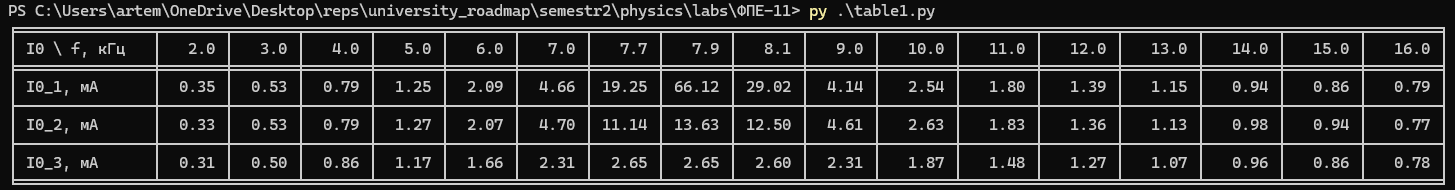
\includegraphics[width=1.0\textwidth]{table1_photo.png}
    \end{figure}

    \vspace{1em}
    \setlength{\parindent}{0pt}

    На основі даних з таблиці №1, було побудовано наступний графік:

    \begin{figure}[ht]
        \includegraphics[width=1.0\textwidth]{Graph1.png}
    \end{figure}

    \setlength{\parindent}{1.5em}

    Отже $I_{0_{max}}$ для $R = 100$ Ом дорівнює $I_{0_{max}} = 13,63 \cdot 10^{-3}$ А. Звідси $I_{0_{max}}/\sqrt{2} = 13,63 \cdot 10^{-3}/\sqrt{2} \approx 9,64 \cdot 10^{-3}$ А = 9,64 мА.
    Значення $I_{0_{max}}$ для $R = 1$ Ом дорівнює $I_{0_{max}} = 66,12 \cdot 10^{-3}$ А. Звідси $I_{0_{max}}/\sqrt{2} = 66,12 \cdot 10^{-3}/\sqrt{2} \approx 46,75 \cdot 10^{-3}$ А = 46,75 мА.

    \vspace{1em}

    Для опору $R = 1$ Ом:

    $f_{\text{рез}} = 7926,61$ Гц, $f_1$ = 7823,39 Гц, $f_2$ = 8009,17 Гц. $\Delta f = f_2 - f_1 = 8009,17 - 7823,39 = 185,78$ Гц.

    Тоді $\displaystyle Q_{R = 1} = \frac{f_{\text{рез}}}{\Delta f} = \frac{7926,61}{185,78} = 42,66$.

    Для опору $R = 500$ Ом:

    $f_{\text{рез}} = 7926,61$ Гц, $f_1$ = 7528,97 Гц, $f_2$ = 8296,64 Гц. $\Delta f = f_2 - f_1 = 8296,64 - 7528,97 = 767,67$ Гц.

    Тоді $\displaystyle Q_{R = 500} = \frac{f_{\text{рез}}}{\Delta f} = \frac{7926,61}{767,67} = 10,32$.

    \vspace{2em}
    \setlength{\parindent}{0pt}

    \textbf{\large Завдання №2:}

    \vspace{1em}

    \begin{table}[h!]

        \centering
        \begin{tabular}{|c|*{10}{c|}}
        \hline
        $C$, нФ & 1 & 2 & 3 & 4 & 5 & 6 & 7 & 8 & 9 & 10 \\
        \hline
        $f_{\text{рез}},~\text{кГц}$ & 13,757 & 9,728 & 7,943 & 6,879 & 6,152 & 5,616 & 5,200 & 4,864 & 4,586 & 4,350 \\
        \hline
        $Z$, $\text{с}^2 \cdot 10^{-10}$ & 1,338 & 2,677 & 4,015 & 5,353 & 6,693 & 8,031 & 9,368 & 10,710 & 12,040 & 13,390 \\
        \hline
        \end{tabular}
        \caption{Розрахунок залежності $f_{\text{рез}}$ та $Z$ від ємності $C$}

    \end{table}

    Обчислення проводились за допомогою Python коду (Лістинг 4.2).

    \newpage

    Результат виконання програми з Лістингу 4.2:

    \begin{figure}[ht]
        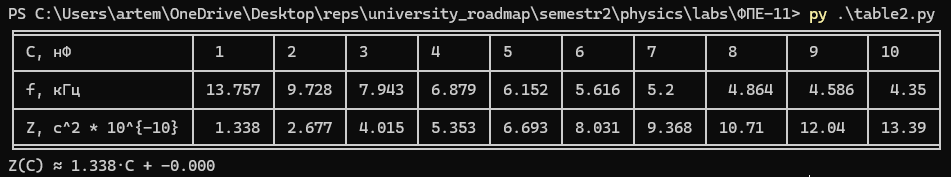
\includegraphics[width=1.0\textwidth]{table2_photo.png}
    \end{figure}

    На основі даних з таблиці №2, було побудовано наступний графік:

    \begin{figure}[ht]
        \includegraphics[width=1.0\textwidth]{Graph2.png}
    \end{figure}

    \setlength{\parindent}{1.5em}

    Чисельне значення тангенсу кута між цією прямою та віссю абсцис дорівнює значенню коефіцієнта нахилу $k$ у рівнянні прямої $y = kx + b$.

    Дані функціональні залежності (для супремуму та інфімуму функції $Z(C)$) знаходились шляхом лінійної регресії, дані для якої були взяті з таблиці №2.
    Значення коефіцієнта нахилу $k$ у рівнянні прямої $y = kx + b$  чисельно дорівнює тангенсу кута між цією прямою та віссю абсцис.

    За результами обчислення, ми отримали, що $Z = Ck + b$, де $k \approx 1,338$. Але так як зліва маємо додатковий множник $10^{-10}$, а справа --- $10^{-9}$, то
    "реальний"  коефіцієнт лінійної регресії дорівнює $k = 0,1338 = 133,8 \cdot 10^{-3}$.

    Відповідно коефіцієнт нахилу для функції інфімуму $Z(C)$ це $k_{sup} = 133,8 \cdot 1,05 \cdot 10^{-3} = 140,49 \cdot 10^{-3}$.
    Коефіцієнт нахилу для функції супремуму $Z(C)$ це $k_{inf} = 133,8 \cdot 0,95 \cdot 10^{-3} = 127,11 \cdot 10^{-3}$.

    Відповідно так як значення індуктивності котушки чисельно дорівнює тангенсу кута між прямою та віссю абсцис, тобто значенню $k$, то відповідно
    $L_1 = k_{inf} = 127,11 \cdot 10^{-3}$ Гн та $L_2 = k_{sup} = 140,49 \cdot 10^{-3}$ Гн.

    Звідси $\displaystyle L_{\text{ср}} = \frac{L_1 + L_2}{2} = \frac{127,11 \cdot 10^{-3} + 140,49 \cdot 10^{-3}}{2} = 133,8 \cdot 10^{-3}$ Гн = 133,8 мГн.

    \vspace{1em}

    Звідси відносна похибка визначення $L$:

    $\displaystyle \varepsilon_L = \frac{\Delta L}{L_{\text{ср}}} \cdot 100\%
    = \frac{L_2 - L_{\text{ср}}}{L_{\text{ср}}} \cdot 100\%
    = \frac{140,49 \cdot 10^{-3} - 133,8 \cdot 10^{-3}}{133,8 \cdot 10^{-3}} \cdot 100\%
    = \frac{6,69 \cdot 10^{-3}}{133,8 \cdot 10^{-3}} \cdot 100\% = 0,05 \cdot 100\% = 5\%$.

    \newpage

    \begin{center}\textbf{\large Обчислення похибок}\end{center}

    \newpage

    \begin{center}
        \textbf{\Large Контрольні запитання}
    \end{center}

    \setlength{\parindent}{0pt}

    \textbf{1. Як виводиться рівняння сталих вимушених коливань у контурі?}

    Електрорушійна сила змінюється гармонічно:
    \[
    \varepsilon = \varepsilon_0 \cos(\Omega t)
    \]
    Згідно з другим законом Кірхгофа:
    \[
    \varepsilon = IR + L\frac{dI}{dt} + \frac{q}{C}
    \]
    Враховуючи, що $\displaystyle I = \frac{dq}{dt}$, після підстановки отримаємо диференціальне рівняння:
    \[
    \frac{d^2q}{dt^2} + 2\beta \frac{dq}{dt} + \omega_0^2 q = \frac{\varepsilon_0}{L} \cos(\Omega t)
    \]
    де $\displaystyle \beta = \frac{R}{2L}$, $\displaystyle \omega_0 = \frac{1}{\sqrt{LC}}$. Це і є рівняння сталих вимушених коливань.

    \vspace{1em}

    \textbf{2. Вивести формулу залежності амплітуди сили струму у коливальному контурі від частоти зовнішньої ЕРС.}

    Загальний вигляд струму:
    \[
    I(t) = I_0 \cos(\Omega t + \varphi)
    \]
    Амплітуда сили струму:
    \[
    I_0 = \frac{\varepsilon_0 \Omega C}{\sqrt{(\omega_0^2 - \Omega^2)^2 + 4\beta^2 \Omega^2}}
    \]

    \vspace{1em}

    \textbf{3. Вивести формулу для розрахунку кута зсуву фаз за допомогою фігур Ліссажу.}

    При подачі синусоїдних сигналів однакової частоти на X і Y-канали осцилографа фігура Ліссажу має вигляд еліпса. Якщо амплітуди рівні, то півосі \( a \) та \( b \) еліпса пов’язані з фазовим зсувом:
    \[
    \tan(2\varphi) = \frac{2b}{a} \quad \Rightarrow \quad \tan\varphi = \frac{b}{a}
    \]

    \vspace{1em}

    \textbf{4. Що називається резонансом?}

    Резонанс у коливальному контурі — це явище різкого зростання амплітуди сили струму при наближенні частоти зовнішньої ЕРС до власної частоти контуру:
    \[
    \Omega \approx \omega_0
    \]

    \vspace{1em}

    \textbf{5. Що таке добротність коливального контуру?}

    Добротність \( Q \) характеризує відношення енергії, накопиченої в контурі, до втрат енергії за один цикл:
    \[
    Q = \frac{\omega_0}{2\beta} = \frac{1}{R} \sqrt{\frac{L}{C}}
    \]

    \vspace{1em}

    \textbf{6. Показати, що резонанс струмів настає за частоти зовнішньої ЕРС \( \omega_0 = \Omega \).}

    З формули амплітуди струму:
    \[
    I_0 = \frac{\varepsilon_0 \Omega C}{\sqrt{(\omega_0^2 - \Omega^2)^2 + 4\beta^2 \Omega^2}}
    \]
    Максимум досягається, коли знаменник мінімальний, тобто:
    \[
    \omega_0 = \Omega
    \]
    що й означає резонанс струму.

\end{document}